\subsection{Paradigm Support}

% good for dynamic
%% composite types are dynamic
Functional and dynamic languages

The groundwork is there, can primitives be used to make support?

\subsection{Performance Analysis}

\subsubsection{Micro Benchmarking}

Heap objects (w/ fields)

Sub-routines

Boxing

General use (stack, algorithms)

Recursion
\begin{figure}[H]
  \centering
  % Created by tikzDevice version 0.8.1 on 2015-06-27 20:39:43
% !TEX encoding = UTF-8 Unicode
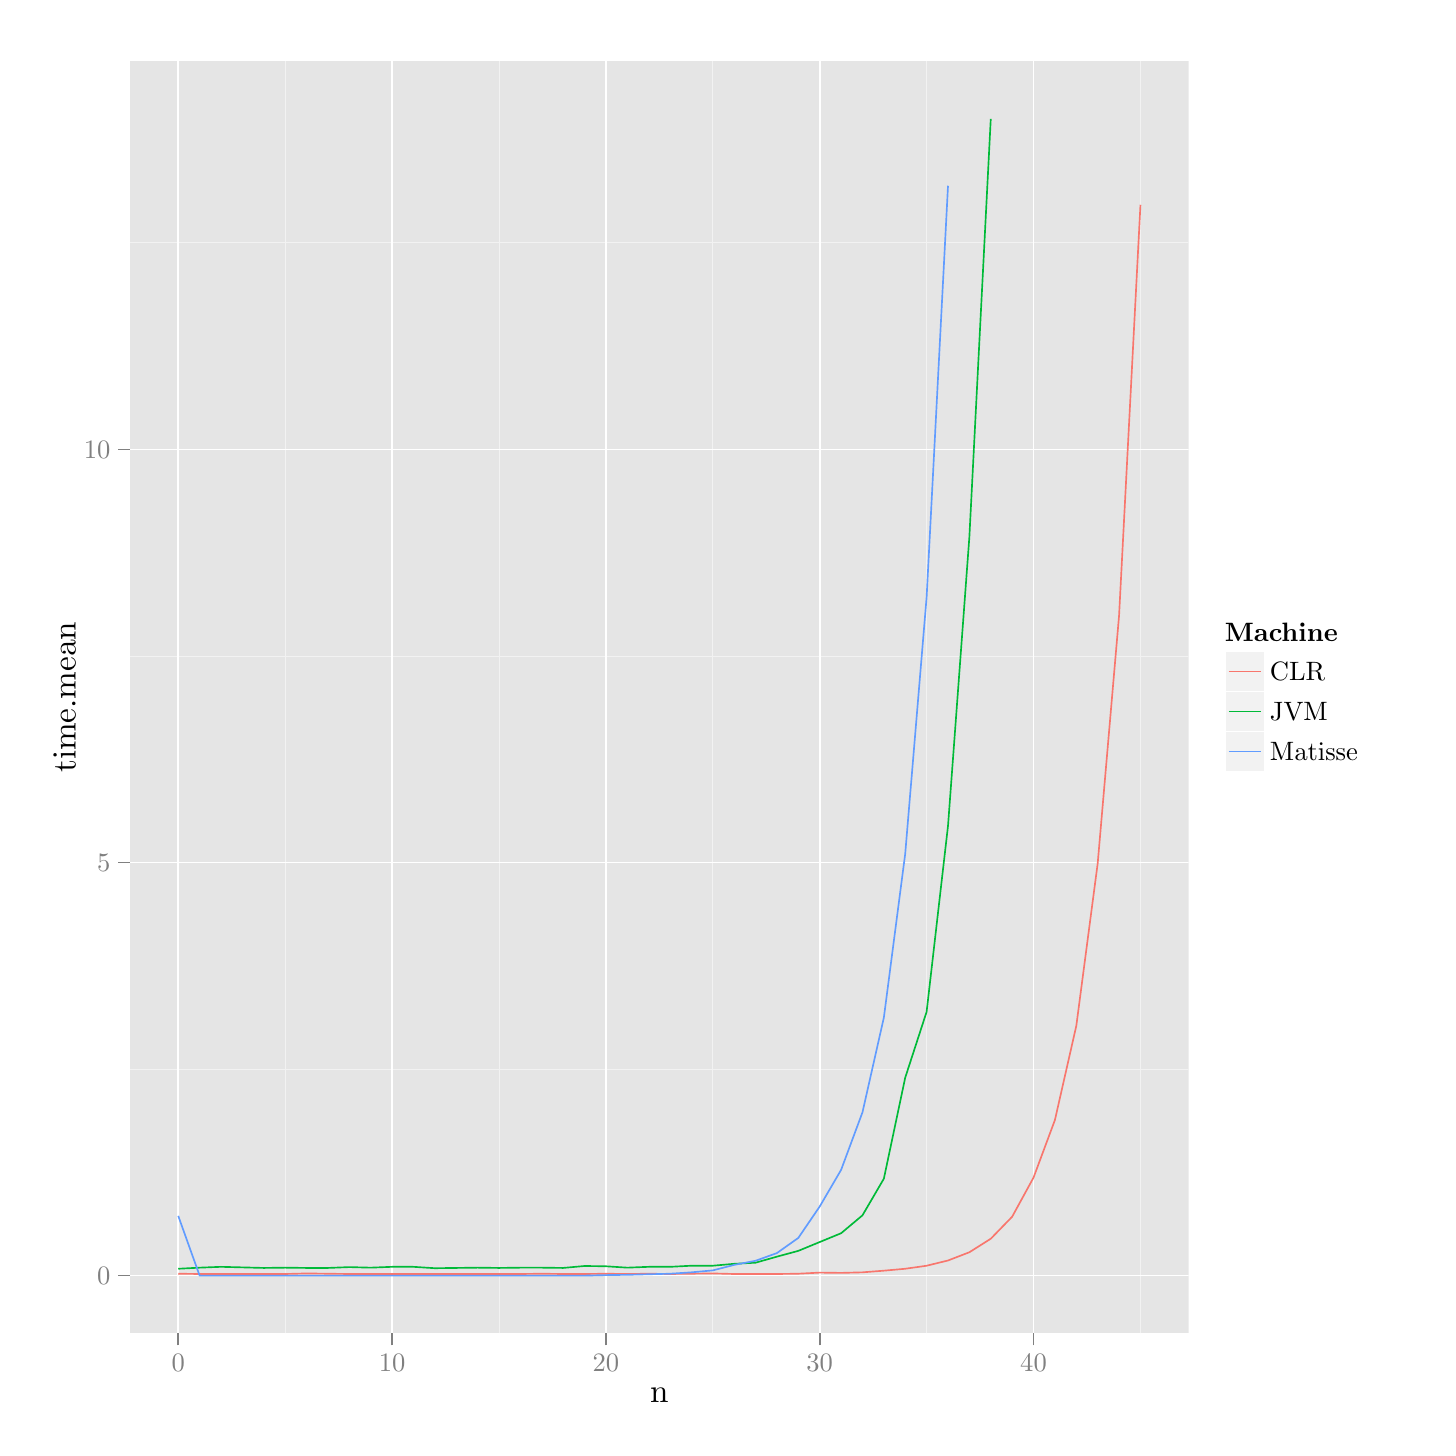
\begin{tikzpicture}[x=1pt,y=1pt]
\definecolor{fillColor}{RGB}{255,255,255}
\path[use as bounding box,fill=fillColor,fill opacity=0.00] (0,0) rectangle (505.89,505.89);
\begin{scope}
\path[clip] (  0.00,  0.00) rectangle (505.89,505.89);
\definecolor{drawColor}{RGB}{255,255,255}
\definecolor{fillColor}{RGB}{255,255,255}

\path[draw=drawColor,line width= 0.6pt,line join=round,line cap=round,fill=fillColor] (  0.00,  0.00) rectangle (505.89,505.89);
\end{scope}
\begin{scope}
\path[clip] ( 37.02, 34.03) rectangle (419.48,493.85);
\definecolor{fillColor}{gray}{0.90}

\path[fill=fillColor] ( 37.02, 34.03) rectangle (419.48,493.85);
\definecolor{drawColor}{gray}{0.95}

\path[draw=drawColor,line width= 0.3pt,line join=round] ( 37.02,129.58) --
	(419.48,129.58);

\path[draw=drawColor,line width= 0.3pt,line join=round] ( 37.02,278.87) --
	(419.48,278.87);

\path[draw=drawColor,line width= 0.3pt,line join=round] ( 37.02,428.16) --
	(419.48,428.16);

\path[draw=drawColor,line width= 0.3pt,line join=round] ( 93.04, 34.03) --
	( 93.04,493.85);

\path[draw=drawColor,line width= 0.3pt,line join=round] (170.30, 34.03) --
	(170.30,493.85);

\path[draw=drawColor,line width= 0.3pt,line join=round] (247.57, 34.03) --
	(247.57,493.85);

\path[draw=drawColor,line width= 0.3pt,line join=round] (324.83, 34.03) --
	(324.83,493.85);

\path[draw=drawColor,line width= 0.3pt,line join=round] (402.10, 34.03) --
	(402.10,493.85);
\definecolor{drawColor}{RGB}{255,255,255}

\path[draw=drawColor,line width= 0.6pt,line join=round] ( 37.02, 54.94) --
	(419.48, 54.94);

\path[draw=drawColor,line width= 0.6pt,line join=round] ( 37.02,204.22) --
	(419.48,204.22);

\path[draw=drawColor,line width= 0.6pt,line join=round] ( 37.02,353.51) --
	(419.48,353.51);

\path[draw=drawColor,line width= 0.6pt,line join=round] ( 54.41, 34.03) --
	( 54.41,493.85);

\path[draw=drawColor,line width= 0.6pt,line join=round] (131.67, 34.03) --
	(131.67,493.85);

\path[draw=drawColor,line width= 0.6pt,line join=round] (208.93, 34.03) --
	(208.93,493.85);

\path[draw=drawColor,line width= 0.6pt,line join=round] (286.20, 34.03) --
	(286.20,493.85);

\path[draw=drawColor,line width= 0.6pt,line join=round] (363.46, 34.03) --
	(363.46,493.85);
\definecolor{drawColor}{RGB}{248,118,109}

\path[draw=drawColor,line width= 0.6pt,line join=round] ( 54.41, 55.63) --
	( 62.13, 55.53) --
	( 69.86, 55.53) --
	( 77.58, 55.53) --
	( 85.31, 55.53) --
	( 93.04, 55.53) --
	(100.76, 55.73) --
	(108.49, 55.63) --
	(116.22, 55.53) --
	(123.94, 55.53) --
	(131.67, 55.53) --
	(139.40, 55.53) --
	(147.12, 55.53) --
	(154.85, 55.53) --
	(162.58, 55.53) --
	(170.30, 55.53) --
	(178.03, 55.53) --
	(185.75, 55.63) --
	(193.48, 55.53) --
	(201.21, 55.53) --
	(208.93, 55.63) --
	(216.66, 55.53) --
	(224.39, 55.63) --
	(232.11, 55.53) --
	(239.84, 55.63) --
	(247.57, 55.73) --
	(255.29, 55.53) --
	(263.02, 55.53) --
	(270.75, 55.53) --
	(278.47, 55.63) --
	(286.20, 56.03) --
	(293.93, 55.93) --
	(301.65, 56.13) --
	(309.38, 56.73) --
	(317.10, 57.42) --
	(324.83, 58.52) --
	(332.56, 60.41) --
	(340.28, 63.39) --
	(348.01, 68.27) --
	(355.74, 76.23) --
	(363.46, 90.37) --
	(371.19,111.17) --
	(378.92,145.21) --
	(386.64,203.83) --
	(394.37,293.40) --
	(402.10,441.89);
\definecolor{drawColor}{RGB}{0,186,56}

\path[draw=drawColor,line width= 0.6pt,line join=round] ( 54.41, 57.42) --
	( 62.13, 57.82) --
	( 69.86, 58.12) --
	( 77.58, 57.92) --
	( 85.31, 57.72) --
	( 93.04, 57.82) --
	(100.76, 57.72) --
	(108.49, 57.72) --
	(116.22, 58.02) --
	(123.94, 57.82) --
	(131.67, 58.12) --
	(139.40, 58.12) --
	(147.12, 57.62) --
	(154.85, 57.72) --
	(162.58, 57.82) --
	(170.30, 57.72) --
	(178.03, 57.82) --
	(185.75, 57.82) --
	(193.48, 57.72) --
	(201.21, 58.42) --
	(208.93, 58.32) --
	(216.66, 57.82) --
	(224.39, 58.12) --
	(232.11, 58.12) --
	(239.84, 58.52) --
	(247.57, 58.52) --
	(255.29, 59.21) --
	(263.02, 59.61) --
	(270.75, 61.80) --
	(278.47, 63.89) --
	(286.20, 67.08) --
	(293.93, 70.26) --
	(301.65, 76.73) --
	(309.38, 89.97) --
	(317.10,126.49) --
	(324.83,150.28) --
	(332.56,217.46) --
	(340.28,321.86) --
	(348.01,472.94);
\definecolor{drawColor}{RGB}{97,156,255}

\path[draw=drawColor,line width= 0.6pt,line join=round] ( 54.41, 76.53) --
	( 62.13, 54.94) --
	( 69.86, 54.94) --
	( 77.58, 54.94) --
	( 85.31, 54.94) --
	( 93.04, 54.94) --
	(100.76, 54.94) --
	(108.49, 54.94) --
	(116.22, 54.94) --
	(123.94, 54.94) --
	(131.67, 54.94) --
	(139.40, 54.94) --
	(147.12, 54.94) --
	(154.85, 54.94) --
	(162.58, 54.94) --
	(170.30, 54.94) --
	(178.03, 54.94) --
	(185.75, 54.94) --
	(193.48, 54.94) --
	(201.21, 54.94) --
	(208.93, 55.13) --
	(216.66, 55.23) --
	(224.39, 55.43) --
	(232.11, 55.63) --
	(239.84, 56.13) --
	(247.57, 56.83) --
	(255.29, 58.82) --
	(263.02, 60.31) --
	(270.75, 63.10) --
	(278.47, 68.57) --
	(286.20, 79.92) --
	(293.93, 93.15) --
	(301.65,113.95) --
	(309.38,148.19) --
	(317.10,207.41) --
	(324.83,300.07) --
	(332.56,448.76);
\end{scope}
\begin{scope}
\path[clip] (  0.00,  0.00) rectangle (505.89,505.89);
\definecolor{drawColor}{gray}{0.50}

\node[text=drawColor,anchor=base east,inner sep=0pt, outer sep=0pt, scale=  0.96] at ( 29.91, 51.63) {0};

\node[text=drawColor,anchor=base east,inner sep=0pt, outer sep=0pt, scale=  0.96] at ( 29.91,200.92) {5};

\node[text=drawColor,anchor=base east,inner sep=0pt, outer sep=0pt, scale=  0.96] at ( 29.91,350.21) {10};
\end{scope}
\begin{scope}
\path[clip] (  0.00,  0.00) rectangle (505.89,505.89);
\definecolor{drawColor}{gray}{0.50}

\path[draw=drawColor,line width= 0.6pt,line join=round] ( 32.75, 54.94) --
	( 37.02, 54.94);

\path[draw=drawColor,line width= 0.6pt,line join=round] ( 32.75,204.22) --
	( 37.02,204.22);

\path[draw=drawColor,line width= 0.6pt,line join=round] ( 32.75,353.51) --
	( 37.02,353.51);
\end{scope}
\begin{scope}
\path[clip] (  0.00,  0.00) rectangle (505.89,505.89);
\definecolor{drawColor}{gray}{0.50}

\path[draw=drawColor,line width= 0.6pt,line join=round] ( 54.41, 29.77) --
	( 54.41, 34.03);

\path[draw=drawColor,line width= 0.6pt,line join=round] (131.67, 29.77) --
	(131.67, 34.03);

\path[draw=drawColor,line width= 0.6pt,line join=round] (208.93, 29.77) --
	(208.93, 34.03);

\path[draw=drawColor,line width= 0.6pt,line join=round] (286.20, 29.77) --
	(286.20, 34.03);

\path[draw=drawColor,line width= 0.6pt,line join=round] (363.46, 29.77) --
	(363.46, 34.03);
\end{scope}
\begin{scope}
\path[clip] (  0.00,  0.00) rectangle (505.89,505.89);
\definecolor{drawColor}{gray}{0.50}

\node[text=drawColor,anchor=base,inner sep=0pt, outer sep=0pt, scale=  0.96] at ( 54.41, 20.31) {0};

\node[text=drawColor,anchor=base,inner sep=0pt, outer sep=0pt, scale=  0.96] at (131.67, 20.31) {10};

\node[text=drawColor,anchor=base,inner sep=0pt, outer sep=0pt, scale=  0.96] at (208.93, 20.31) {20};

\node[text=drawColor,anchor=base,inner sep=0pt, outer sep=0pt, scale=  0.96] at (286.20, 20.31) {30};

\node[text=drawColor,anchor=base,inner sep=0pt, outer sep=0pt, scale=  0.96] at (363.46, 20.31) {40};
\end{scope}
\begin{scope}
\path[clip] (  0.00,  0.00) rectangle (505.89,505.89);
\definecolor{drawColor}{RGB}{0,0,0}

\node[text=drawColor,anchor=base,inner sep=0pt, outer sep=0pt, scale=  1.20] at (228.25,  9.03) {n};
\end{scope}
\begin{scope}
\path[clip] (  0.00,  0.00) rectangle (505.89,505.89);
\definecolor{drawColor}{RGB}{0,0,0}

\node[text=drawColor,rotate= 90.00,anchor=base,inner sep=0pt, outer sep=0pt, scale=  1.20] at ( 17.30,263.94) {time.mean};
\end{scope}
\begin{scope}
\path[clip] (  0.00,  0.00) rectangle (505.89,505.89);
\definecolor{fillColor}{RGB}{255,255,255}

\path[fill=fillColor] (428.35,232.87) rectangle (484.98,295.01);
\end{scope}
\begin{scope}
\path[clip] (  0.00,  0.00) rectangle (505.89,505.89);
\definecolor{drawColor}{RGB}{0,0,0}

\node[text=drawColor,anchor=base west,inner sep=0pt, outer sep=0pt, scale=  0.96] at (432.62,284.11) {\bfseries Machine};
\end{scope}
\begin{scope}
\path[clip] (  0.00,  0.00) rectangle (505.89,505.89);
\definecolor{drawColor}{RGB}{255,255,255}
\definecolor{fillColor}{gray}{0.95}

\path[draw=drawColor,line width= 0.6pt,line join=round,line cap=round,fill=fillColor] (432.62,266.05) rectangle (447.07,280.50);
\end{scope}
\begin{scope}
\path[clip] (  0.00,  0.00) rectangle (505.89,505.89);
\definecolor{drawColor}{RGB}{248,118,109}

\path[draw=drawColor,line width= 0.6pt,line join=round] (434.06,273.27) -- (445.62,273.27);
\end{scope}
\begin{scope}
\path[clip] (  0.00,  0.00) rectangle (505.89,505.89);
\definecolor{drawColor}{RGB}{255,255,255}
\definecolor{fillColor}{gray}{0.95}

\path[draw=drawColor,line width= 0.6pt,line join=round,line cap=round,fill=fillColor] (432.62,251.59) rectangle (447.07,266.05);
\end{scope}
\begin{scope}
\path[clip] (  0.00,  0.00) rectangle (505.89,505.89);
\definecolor{drawColor}{RGB}{0,186,56}

\path[draw=drawColor,line width= 0.6pt,line join=round] (434.06,258.82) -- (445.62,258.82);
\end{scope}
\begin{scope}
\path[clip] (  0.00,  0.00) rectangle (505.89,505.89);
\definecolor{drawColor}{RGB}{255,255,255}
\definecolor{fillColor}{gray}{0.95}

\path[draw=drawColor,line width= 0.6pt,line join=round,line cap=round,fill=fillColor] (432.62,237.14) rectangle (447.07,251.59);
\end{scope}
\begin{scope}
\path[clip] (  0.00,  0.00) rectangle (505.89,505.89);
\definecolor{drawColor}{RGB}{97,156,255}

\path[draw=drawColor,line width= 0.6pt,line join=round] (434.06,244.37) -- (445.62,244.37);
\end{scope}
\begin{scope}
\path[clip] (  0.00,  0.00) rectangle (505.89,505.89);
\definecolor{drawColor}{RGB}{0,0,0}

\node[text=drawColor,anchor=base west,inner sep=0pt, outer sep=0pt, scale=  0.96] at (448.88,269.97) {CLR};
\end{scope}
\begin{scope}
\path[clip] (  0.00,  0.00) rectangle (505.89,505.89);
\definecolor{drawColor}{RGB}{0,0,0}

\node[text=drawColor,anchor=base west,inner sep=0pt, outer sep=0pt, scale=  0.96] at (448.88,255.51) {JVM};
\end{scope}
\begin{scope}
\path[clip] (  0.00,  0.00) rectangle (505.89,505.89);
\definecolor{drawColor}{RGB}{0,0,0}

\node[text=drawColor,anchor=base west,inner sep=0pt, outer sep=0pt, scale=  0.96] at (448.88,241.06) {Matisse};
\end{scope}
\end{tikzpicture}

  \caption{Mean running time of $Fibonacci(n)$, with $n = 0..35$}
\end{figure}

\subsubsection{Comparison with Existing Systems}

``Indentical'' programs in JVM, CIL

Tables, graphs

\subsubsection{Memory Footprint}

\subsubsection{Optimization}

During the majority of the development we did not concern ourselves with
algorithmic optimization, but rather focused on designing suitable data
structures and writing maintainable and concise code that we would be able to
cope with the inevitable changes during the course of the project. As Rob Pike
states it in his first Rule of Programming: ``You can't tell where a program is
going to spend its time.''\cite{pike-rules}. When the machine had reached a
maturity level that assured us that no further major changes to the overarching
design were necessary we started to analyze the code at a much more detailed
level.

Memory leaks are extremely difficult to avoid when writing any non-trivial C
code. One has to meticulously track allocated memory chunks and free them at
just the right time and place to prevent invalid read and writes. The fact that
C largely does not care about what some collection of bytes represents and
allows virtually any casting does not make this easier. One-off errors are very
common when dealing with arrays and pointers which are indeed a central part of
the \thename{} implementation. Luckily there are tools available to aid in
profiling and pinpointing problematic parts of the code. The absolutely
brilliant instrumentation tool Valgrind\footnote{Valgrind:
  \url{http://valgrind.org}} has been an invaluable help in detecting memory
errors and have allowed us to fix, to our knowledge, all problematic leaks.

Valgrind consists of several different tools that analyzes different things such
as threads, stack operations, caches and memory. We have used the memory error
detector called Memcheck. When an executable is run through Valgrind it is able
to track allocations and the corresponding releases made during the entire
execution. If an allocation does not have exactly one corresponding free
operation it is either a leak or a double free (when the same memory region is
attempted to be release more than once).

The output from Memcheck includes a list of errors and a summary of the leaked
amount of memory. When we initially ran Valgrind with the fibonacci test program
(with $n=15$) the leak summary was this:

\begin{verbatim}
==32067== LEAK SUMMARY:
==32067==    definitely lost: 410,033 bytes in 13,187 blocks
==32067==    indirectly lost: 371,808 bytes in 365 blocks
...
==32067== ERROR SUMMARY: 10 errors from 10 contexts (suppressed: 0 from 0)
\end{verbatim}

This says that there are 10 distinct errors causing a total leak of 400kB
memory, which is a very significant amount of memory for such a small and simple
program. Optimally there should be no bytes leaked at all. Valgrind also tells
you exactly where errors are introduced:

\begin{verbatim}
...
==32067== 27,608 bytes in 986 blocks are definitely lost in loss record 4 of 15
==32067==    at 0x4C29F90: malloc (in /usr/lib/valgrind/vgpreload_memcheck-amd64-linux.so)
==32067==    by 0x4018F4: stack_create_element (stack.c:128)
...
\end{verbatim}

An allocation is being made in the function \code{stack\_create\_element} and is
not released when the program exits. In this case we were not properly releasing
temporary stack elements. Being aware of the issue we changed the way stack
elements were created and the result was a sum total of 40 bytes leaked all of
which are test data structures that are irrelevant for the actual performance
analysis.

The other form of profiling we did was by use of the equally wonderful tool
called gprof\footnote{GNU gprof:
  \url{https://sourceware.org/binutils/docs/gprof/}} (for GNU profiler). It
works in a somewhat different way than Valgrind: executables are compiled with a
special profiling flag that injects profiling code into the binary. When the
file is executed it generates data that is then run through gprof that performs
the analysis. The output is a detailed overview of the CPU time spent in each
function. It is important to avoid profiling optimized binaries because some
crucial information can be lost during when the compiler performs various code
transformations. For example, if the compiler inlines a function into another,
the former will appear to be using the resources that are actually spent by the
inlined function.

As an example of how we used gprof to pinpoint bottlenecks, an initial analysis
showed that 9\% of the total running time was spent in the function
\code{bytes2int} which converts a sequence of bytes into an integral C value. It
is a frequent operation but we found it is suspicious to be using almost one
tenth of the total CPU resources. It was indeed not optimally
implemented; Listing~\ref{lst:eval:gprof-pre} and~\ref{lst:eval:gprof-post}
shows the specific code before and after optimization.

\begin{lstlisting}[language={[ANSI]C},%
  caption={The function \code{bytes2int} before optimization.},%
  label={lst:eval:gprof-pre}]
int64_t value = 0;
int i = size;
while (i) {
    value += ((int64_t) bytes[i - 1]) << (8 * (size - i));
    i--;
}
return value;
\end{lstlisting}

\begin{lstlisting}[language={[ANSI]C},%
  caption={The function \code{bytes2int} after optimization},%
  label={lst:eval:gprof-post}]
switch (size) {
case 1: return bytes[0];
case 2: return bytes[1] | bytes[0] << 8;
case 4: return __builtin_bswap32(*(int32_t*)bytes);
case 8: return __builtin_bswap64(*(int64_t*)bytes);
default: return 0;
}
\end{lstlisting}

The optimized version of the function clocked in at the much better 1.4\% CPU
time. Using this technique of measuring, pinpointing, patching and measuring
again we managed to more than triple the speed of some test programs! Currently
the bottleneck of the machine seems to lie somewhere in the stack
implementation, as shown in the following gprof output:

\begin{verbatim}
  %   cumulative   self              self     total
 time   seconds   seconds    calls  ms/call  ms/call  name
 20.24      0.52     0.52 35002981     0.00     0.00  am_exec_instr
  8.17      0.73     0.21 24232831     0.00     0.00  stack_segment_push_element
  6.62      0.90     0.17 35002981     0.00     0.00  am_read_prefixes
  5.64      1.05     0.15 24232831     0.00     0.00  stack_push
  5.06      1.18     0.13 17501491     0.00     0.00  stack_peek
...
\end{verbatim}

Generally it is difficult to determine whether there is a problem with a part of
the code or if it is just a frequent operation in the specific
program. Profiling multiple test programs that utilize different features can
reveal common bottlenecks which should be analyzed further.

Whether there are more fundamental architectural design issues that limits
performance is difficult to say. We have not encountered major issues with how
the modules interoperate.

\subsection{Code Analysis}
\subsubsection{Code size (SLOC)}
\subsubsection{Architectural analysis}
\subsubsection{Readability, maintainability}
\subsubsection{Tests, coverage}
\subsubsection{Configurability (macros)}

\subsection{Documentation}

Very brief doxy description

% Usage evaluation
%% Have the problems been solved

% Assembly generation
%% Something about generating code for the machine

% Performance
%% Function calls
%% Analysis

% Future development
%% What's missing
%% What could be different
%% What would next steps be

%%% Local Variables:
%%% mode: latex
%%% TeX-master: "../report"
%%% End:
